\documentclass[11pt,a4paper]{article}

\usepackage[utf8]{inputenc}
\usepackage[T1]{fontenc}
\usepackage[french]{babel}
\usepackage[margin=1.8cm]{geometry}
\usepackage{array}
\usepackage{longtable}
\usepackage{booktabs}
\usepackage{tabularx}
\usepackage{xcolor}
\usepackage{colortbl}
\usepackage{enumitem}
\usepackage{titlesec}
\usepackage{graphicx}
\usepackage{float}
\usepackage{amsmath}

\definecolor{titleblue}{RGB}{0,102,153}
\definecolor{lightgray}{RGB}{240,240,240}
\newcolumntype{P}[1]{>{\raggedright\arraybackslash}p{#1}}
\setlength{\parskip}{0.35em}
\setlength{\parindent}{0pt}
\renewcommand{\arraystretch}{1.25}

\titleformat{\section}{\large\bfseries\color{titleblue}}{\thesection}{0.6em}{}
\titleformat{\subsection}{\normalsize\bfseries}{\thesubsection}{0.6em}{}

\begin{document}

\begin{center}
    {\LARGE\bfseries Analyse C1 et C2 de l'API bancaire FastAPI}\\[0.25cm]
    {\large Graphes de flot de contrôle et complexité cyclomatique}\\[0.5cm]
\end{center}

\textbf{Projet :} Système de transaction bancaire\\
\textbf{Étudiant :} KOA ESSAMA PAULIN BRICE\\
\textbf{Matricule :} 25I2255\\
\textbf{Dépôt GitHub :} \texttt{eliote-geeks/Devoir\_304}\\
\textbf{Code source analysé :} \texttt{app/main.py} et \texttt{app/storage.py}

\section{Fonctionnalités du logiciel}

Les cinq fonctions de base analysées à partir du code source sont :

\begin{enumerate}[leftmargin=1.2cm]
    \item \textbf{Créer un compte bancaire}
    \item \textbf{Lister les comptes bancaires}
    \item \textbf{Consulter un compte bancaire}
    \item \textbf{Effectuer un dépôt}
    \item \textbf{Effectuer un retrait}
\end{enumerate}

\textbf{Remarque :} le projet contient aussi une fonction supplémentaire de \textbf{virement entre comptes}, mais l'analyse ci-dessous reste centrée sur les cinq fonctions de base demandées dans le devoir.

\section{Rappel sur C1 et C2}

\textbf{C1} : couverture des instructions. Chaque instruction doit être exécutée au moins une fois.\\
\textbf{C2} : couverture des décisions. Chaque décision doit être testée à \texttt{vrai} et à \texttt{faux}.

\section{Complexité cyclomatique}

La complexité cyclomatique est estimée à partir du graphe de flot de contrôle simplifié :

\[
M = D + 1
\]

où \(D\) est le nombre de décisions du graphe.

\begin{longtable}{|P{4.2cm}|P{2.7cm}|P{3cm}|P{5.4cm}|}
\hline
\rowcolor{lightgray}
\textbf{Fonction} & \textbf{Décisions} & \textbf{Complexité \(M\)} & \textbf{Interprétation} \\
\hline
Créer un compte & 1 & 2 & Deux chemins : avec ou sans dépôt initial. \\
\hline
Lister les comptes & 0 & 1 & Chemin séquentiel unique. \\
\hline
Consulter un compte & 1 & 2 & Deux chemins : compte trouvé ou introuvable. \\
\hline
Effectuer un dépôt & 1 & 2 & Deux chemins : compte trouvé ou introuvable. \\
\hline
Effectuer un retrait & 2 & 3 & Trois chemins : compte introuvable, solde insuffisant, retrait valide. \\
\hline
\end{longtable}

\section{Graphes de flot de contrôle}

\subsection{Fonction 1 : créer un compte}

\begin{figure}[H]
\centering
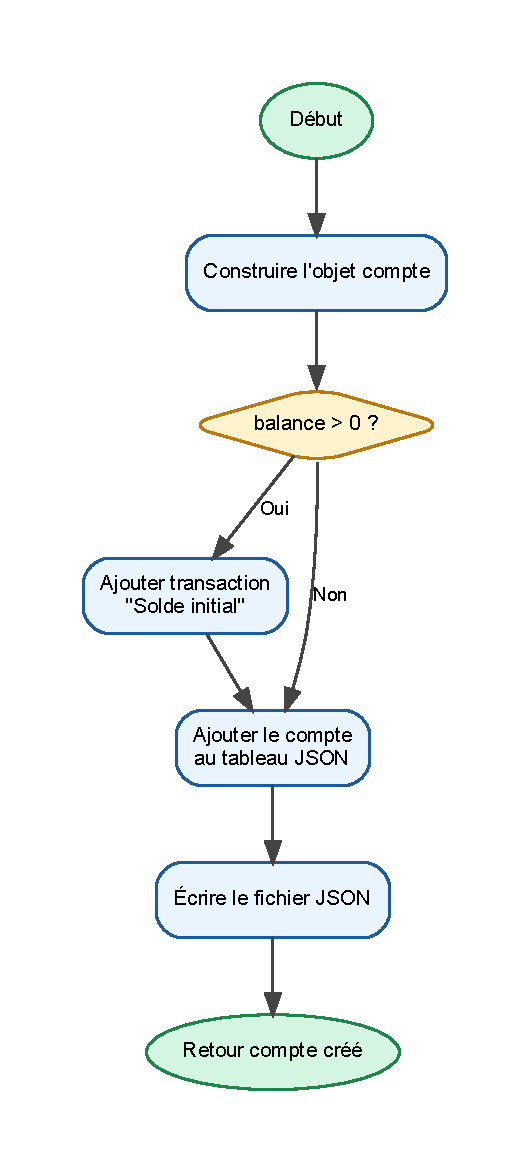
\includegraphics[width=0.62\textwidth]{docs/graphs/create_account.pdf}
\caption{Graphe de flot de contrôle de la création de compte}
\end{figure}

\textbf{Chemins}
\begin{itemize}[leftmargin=1cm]
    \item P1 : création du compte avec \texttt{balance = 0}, sans transaction initiale.
    \item P2 : création du compte avec \texttt{balance > 0}, puis ajout d'une transaction \texttt{deposit}.
\end{itemize}

\subsection{Fonction 2 : lister les comptes}

\begin{figure}[H]
\centering
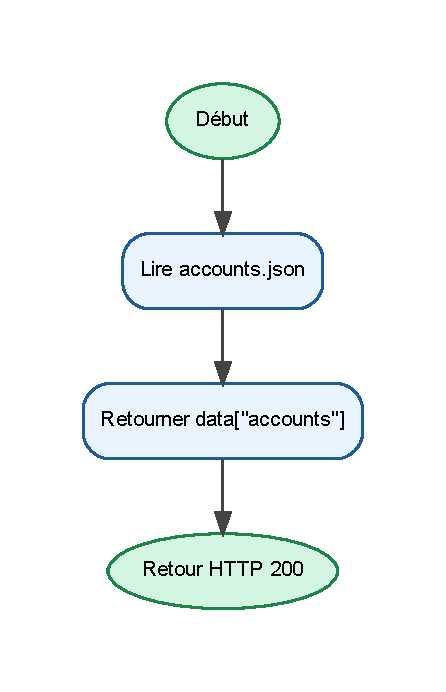
\includegraphics[width=0.48\textwidth]{docs/graphs/list_accounts.pdf}
\caption{Graphe de flot de contrôle de la liste des comptes}
\end{figure}

\textbf{Chemin}
\begin{itemize}[leftmargin=1cm]
    \item P1 : lecture du fichier JSON puis retour de la liste.
\end{itemize}

\subsection{Fonction 3 : consulter un compte}

\begin{figure}[H]
\centering
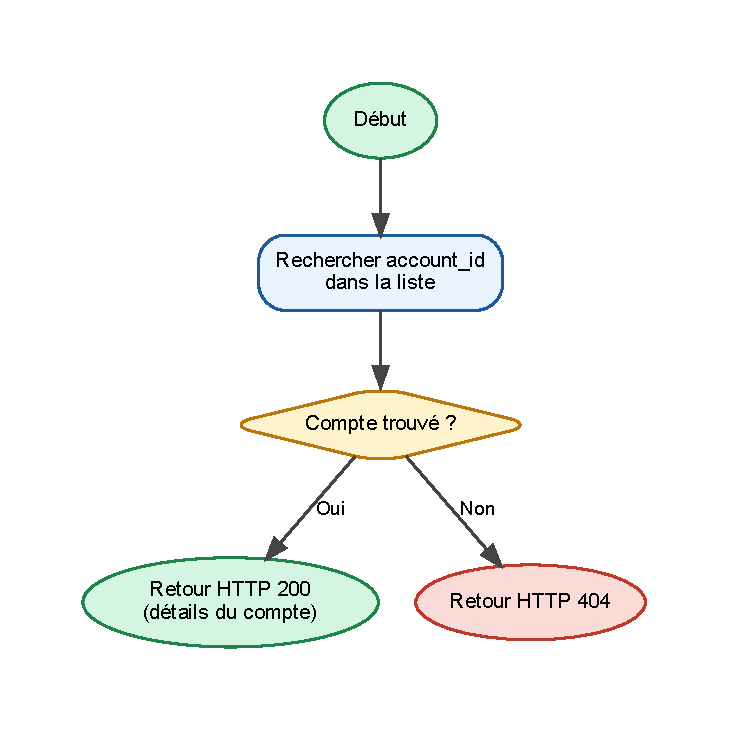
\includegraphics[width=0.58\textwidth]{docs/graphs/get_account.pdf}
\caption{Graphe de flot de contrôle de la consultation d'un compte}
\end{figure}

\textbf{Chemins}
\begin{itemize}[leftmargin=1cm]
    \item P1 : le compte existe, retour HTTP 200.
    \item P2 : le compte n'existe pas, retour HTTP 404.
\end{itemize}

\subsection{Fonction 4 : effectuer un dépôt}

\begin{figure}[H]
\centering
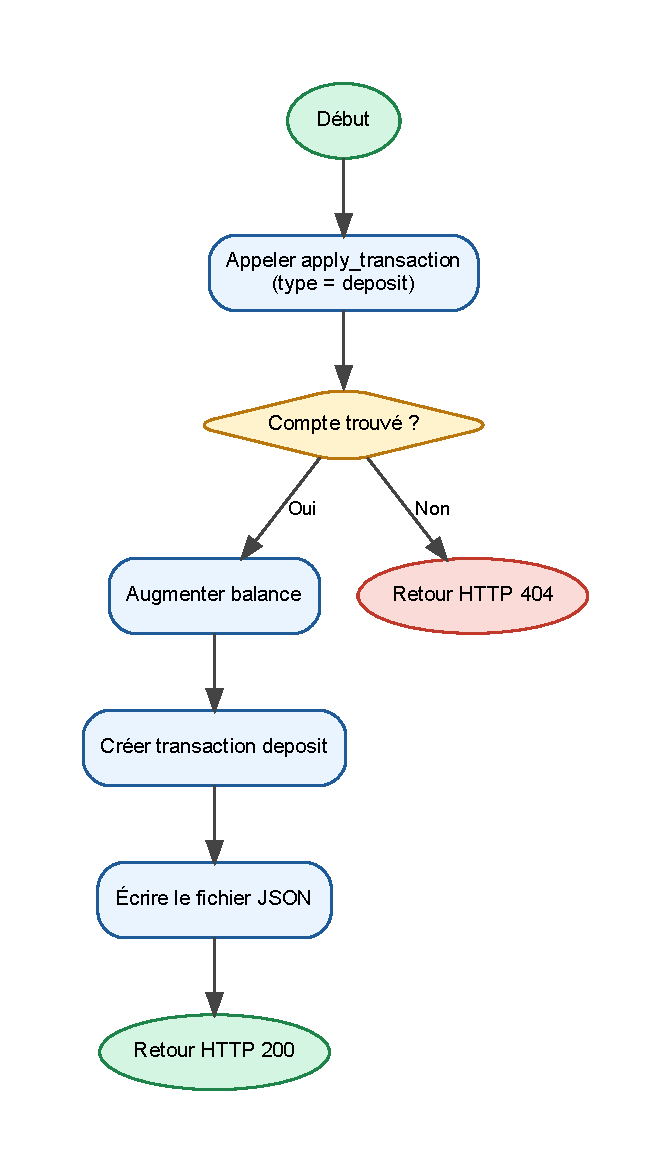
\includegraphics[width=0.66\textwidth]{docs/graphs/deposit.pdf}
\caption{Graphe de flot de contrôle du dépôt}
\end{figure}

\textbf{Chemins}
\begin{itemize}[leftmargin=1cm]
    \item P1 : le compte existe, le solde est augmenté et la transaction est enregistrée.
    \item P2 : le compte est introuvable, retour HTTP 404.
\end{itemize}

\textbf{Observation :} la validation des montants strictement positifs est gérée par Pydantic avant l'exécution de la fonction Python ; elle produit une erreur HTTP 422 mais ne fait pas partie du flot interne de la fonction.

\subsection{Fonction 5 : effectuer un retrait}

\begin{figure}[H]
\centering
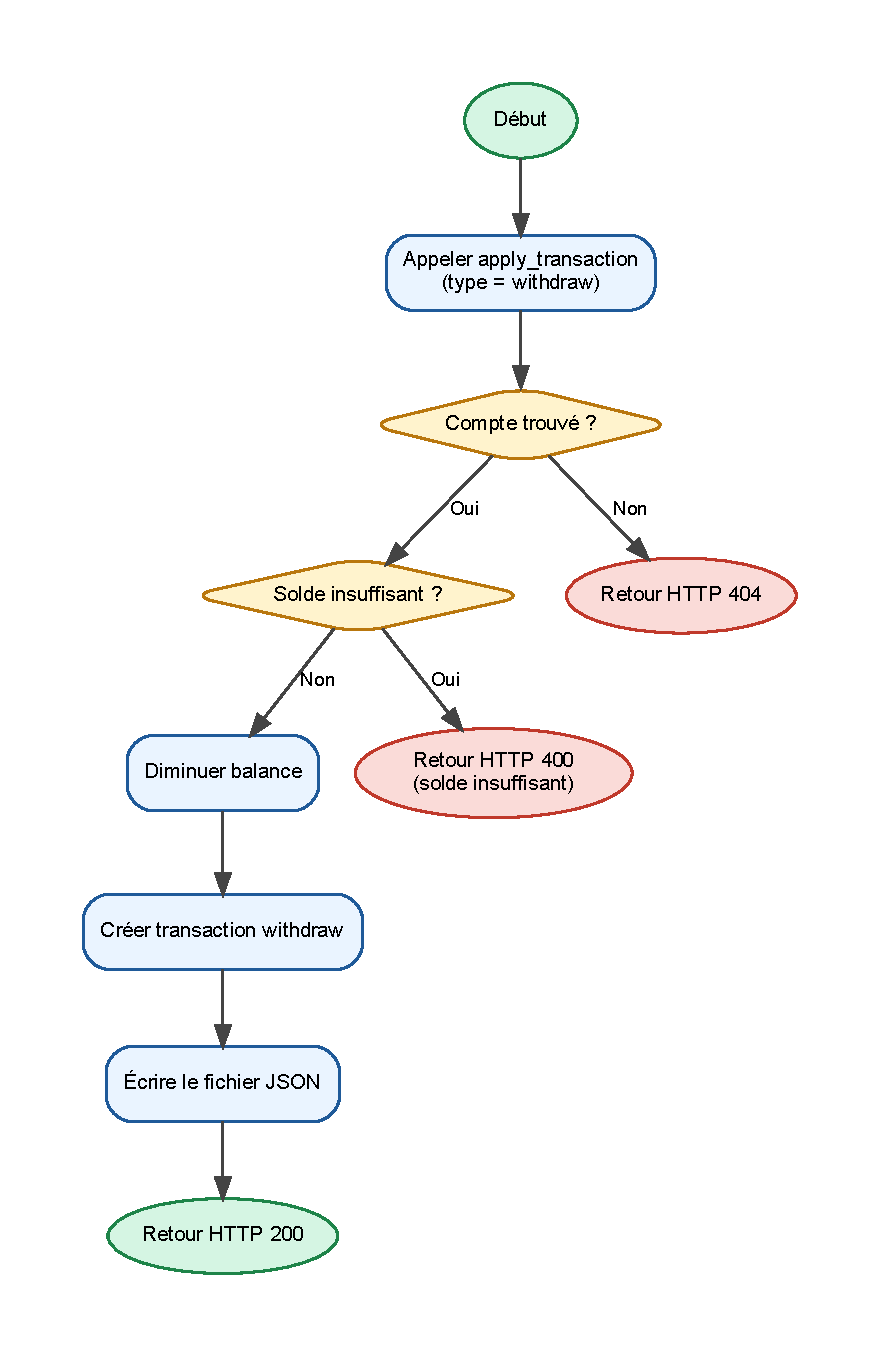
\includegraphics[width=0.7\textwidth]{docs/graphs/withdraw.pdf}
\caption{Graphe de flot de contrôle du retrait}
\end{figure}

\textbf{Chemins}
\begin{itemize}[leftmargin=1cm]
    \item P1 : le compte n'existe pas, retour HTTP 404.
    \item P2 : le compte existe mais le solde est insuffisant, retour HTTP 400.
    \item P3 : le compte existe et le solde est suffisant, mise à jour du solde et retour HTTP 200.
\end{itemize}

\section{Table de progression de couverture}

\begin{longtable}{|P{4.2cm}|P{4.2cm}|P{4.2cm}|P{3.2cm}|}
\hline
\rowcolor{lightgray}
\textbf{Fonction} & \textbf{Tests minimaux pour C1} & \textbf{Tests minimaux pour C2} & \textbf{Couverture obtenue} \\
\hline
Créer un compte & compte avec solde nul + compte avec solde positif & idem & C1 et C2 atteints \\
\hline
Lister les comptes & appel simple de la liste & appel simple de la liste & C1 atteint \\
\hline
Consulter un compte & compte existant + compte inexistant & idem & C1 et C2 atteints \\
\hline
Effectuer un dépôt & dépôt valide + compte inexistant & idem & C1 et C2 atteints \\
\hline
Effectuer un retrait & retrait valide + solde insuffisant + compte inexistant & idem & C1 et C2 atteints \\
\hline
\end{longtable}

\section{Conclusion}

L'analyse du code source montre que les fonctions \texttt{create\_account} et \texttt{withdraw\_money/apply\_transaction} sont les plus intéressantes pour le test structurel. La création de compte introduit un branchement sur le dépôt initial, tandis que le retrait comporte plusieurs chemins d'exécution liés à l'existence du compte et à la suffisance du solde.

Les graphes visuels fournis dans ce document permettent donc de :
\begin{itemize}[leftmargin=1cm]
    \item représenter clairement le flot de contrôle ;
    \item identifier les chemins indépendants ;
    \item calculer la complexité cyclomatique ;
    \item déduire les jeux de tests nécessaires pour C1 et C2.
\end{itemize}

\end{document}
